\lecture{Graphs}{17:00}{12/03/24}{Janka Chlebikova}

\section*{Graphs}

A graph, $G$, is a pair $(V, E)$ of sets, $V$ being the set of vertices and $E$ being the set of edges. Each edge,
 $e \in E$ is denoted either by a set of vertices, e.g. $\{v_1, v_2\}$ or in shorthand as $v_1v_2$, from the set $V$.
 Each edge connects a distinct set of vertices from $V$. The vertices $v_1$ and $v_2$ are said to be incident with the
 edge $v_1v_2$, and are adjacent to each other.

\begin{minipage}[c]{0.3\linewidth}
  \begin{figure}[H]
    \centering
    \usetikzlibrary{graphs}
    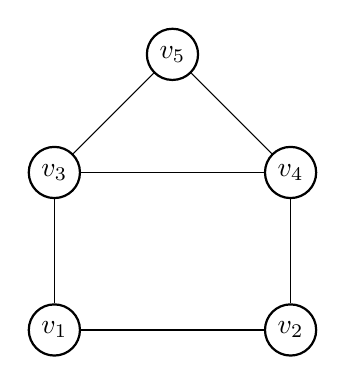
\begin{tikzpicture}
      \tikzset{
        node distance=1.5cm,
        every node/.style={circle,thick,draw,inner sep=0pt,minimum size=6.5mm}
      }
  
      \node[] (v5) {$v_5$};
      \node[right of=v5, below of=v5] (v4) {$v_4$};
      \node[left of=v5, below of=v5] (v3) {$v_3$};
      \node[below of=v4, node distance=2cm] (v2) {$v_2$};
      \node[below of=v3, node distance=2cm] (v1) {$v_1$};
  
      \draw (v1) edge[right] (v2)
            (v1) edge[above] (v3)
            (v2) edge[above] (v4)
            (v3) edge[right] (v4)
            (v3) edge[above] (v5)
            (v4) edge[above] (v5);
    \end{tikzpicture}
    \caption{A graph with 5 vertices and 6 edges}
    \label{fig:graph1}
  \end{figure}
\end{minipage}\hfill
\begin{minipage}{0.6\linewidth}
In the case of the graph in figure \ref*{fig:graph1},\\
$V = \{v_1, v_2, v_3, v_4, v_5\}$\\
$E = \{\{v_1, v_2\}, \{v_1, v_3\}, \{v_2, v_4\}, \{v_3, v_4\}, \{v_3, v_5\}, \{v_4, v_5\}\}$, or\\
$E = \{v_1v_2, v_1v_3, v_2v_4, v_3v_4, v_3v_5, v_4,v_5\}$
\end{minipage}

\subsection*{Multi/Pseudo-Graphs}

A pesudograph, or multigraph, is a graph containing either an edge that connects a vertex to itself, or forms a `loop'
 with two or more edges which connect the same two vertices together. These are not technically graphs, but will still
 be used in this course as they have some properties which are important to understanding graphs as a whole.

\subsection*{Vertices}

There are several properties of vertices, but the one we are most interested in is the \textit{degree} of the vertex. In
 the case of a graph, the degree of a vertex is the number of edges connected to it. This is denoted by $\mathrm{deg}(v_1)$,
 and a vertex with a degree of $0$ is known as `isolated'.

\begin{minipage}[c]{0.35\linewidth}
  \begin{figure}[H]
    \centering
    \usetikzlibrary{graphs}
    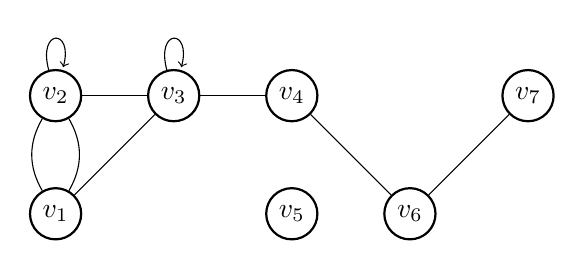
\begin{tikzpicture}
      \tikzset{
        node distance=1.5cm,
        every node/.style={circle,thick,draw,inner sep=0pt,minimum size=6.5mm}
      }

      \node[] (v2) {$v_2$};
      \node[below of=v2] (v1) {$v_1$};
      \node[right of=v2] (v3) {$v_3$};
      \node[right of=v3] (v4) {$v_4$};
      \node[below of=v4] (v5) {$v_5$};
      \node[right of=v4, below of=v4] (v6) {$v_6$};
      \node[right of=v6, above of=v6] (v7) {$v_7$};
  
      \draw (v1) edge[bend right] (v2)
            (v1) edge[bend left] (v2)
            (v1) edge[] (v3)
            (v2) edge[loop above] (v2)
            (v2) edge[] (v3)
            (v3) edge[loop above] (v3)
            (v3) edge[] (v4)
            (v4) edge[] (v6)
            (v6) edge[] (v7);
    \end{tikzpicture}
    \caption{A graph with 7 vertices and 9 edges}
    \label{fig:graph2}
  \end{figure}
\end{minipage}\hfill
\begin{minipage}{0.55\linewidth}
For figure \ref*{fig:graph2}, the degree of each node is as follows:
$\mathrm{deg\ } v_1 = 3$\\
$\mathrm{deg\ } v_2 = 5$\\
$\mathrm{deg\ } v_3 = 5$\\
$\mathrm{deg\ } v_4 = 2$\\
$\mathrm{deg\ } v_5 = 0$\\
$\mathrm{deg\ } v_6 = 6$\\
$\mathrm{deg\ } v_7 = 1$\\
\end{minipage}

When $d_1, d_2, \dots, \d_n$ are the degrees of the vertices in a graph $G$ and $d_1 \leq d_2 \leq \ldots \leq d_n$, the
 degree sequence of $G$ would be $(d_1, d_2, \dots, d_n)$. For example, the degree sequence of the graph in figure
 \ref*{fig:graph2} would be $(0, 1, 2, 3, 5, 5, 6)$.

\subsection*{Euler Theorem}

Euler's Theorem (sometimes known as the Handshaking lemma) states:
\begin{center}
  In any graph, $G = (V, E)$, the sum of all vertex-degrees is equal to twice the number of edges,\\
  $\sum_{v \in V} \mathrm{deg\ } v = 2 \lvert E \rvert$
\end{center}

This has several consequences, namely
\begin{itemize}
  \item The sum of all vertex-degrees is an even number
  \item Adding a single edge increases the degree of 2 vertices by $1$
  \item The number of vertices with odd degrees must be even
\end{itemize}

\section*{Special Graphs}

\subsection*{Complete Graphs}

For any positive integer, $n \in \mathbb{N}$, the complete graph with $n$ vertices, denoted by $K_n$ is the graph in
 which every pair of vertices are adjacent. More simply, every vertex is connected to every other vertex.

\begin{minipage}[c]{0.2\linewidth}
  \begin{figure}[H]
    \centering
    \usetikzlibrary{graphs}
    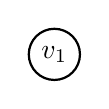
\begin{tikzpicture}
      \tikzset{
        node distance=1.5cm,
        every node/.style={circle,thick,draw,inner sep=0pt,minimum size=6.5mm}
      }
  
      \node[] (v1) {$v_1$};
    \end{tikzpicture}
    \caption{$K_1$}
    \label{fig:graphk1}
  \end{figure}
\end{minipage}\hfill
\begin{minipage}[c]{0.2\linewidth}
  \begin{figure}[H]
    \centering
    \usetikzlibrary{graphs}
    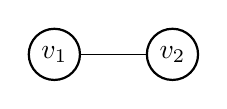
\begin{tikzpicture}
      \tikzset{
        node distance=1.5cm,
        every node/.style={circle,thick,draw,inner sep=0pt,minimum size=6.5mm}
      }
  
      \node[] (v1) {$v_1$};
      \node[right of=v1] (v2) {$v_2$};

      \draw (v1) edge (v2);
    \end{tikzpicture}
    \caption{$K_2$}
    \label{fig:graphk2}
  \end{figure}
\end{minipage}\hfill
\begin{minipage}[c]{0.2\linewidth}
  \begin{figure}[H]
    \centering
    \usetikzlibrary{graphs, positioning, calc}
    \begin{tikzpicture}
      \tikzset{
        node distance=1.5cm,
        every node/.style={circle,thick,draw,inner sep=0pt,minimum size=6.5mm}
      }
  
      \node[] (v1) {$v_1$};
      \node[right of=v1] (v2) {$v_2$};
      \node[yshift=-0.5cm] (v3) [above=of $(v1)!0.5!(v2)$] {$v_3$};

      \draw (v1) edge[] (v2)
            (v2) edge[] (v3)
            (v3) edge[] (v1);
    \end{tikzpicture}
    \caption{$K_3$}
    \label{fig:graphk3}
  \end{figure}
\end{minipage}\hfill
\begin{minipage}[c]{0.2\linewidth}
  \begin{figure}[H]
    \centering
    \usetikzlibrary{graphs}
    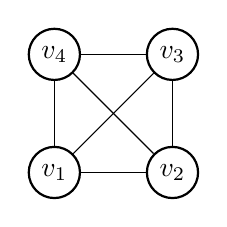
\begin{tikzpicture}
      \tikzset{
        node distance=1.5cm,
        every node/.style={circle,thick,draw,inner sep=0pt,minimum size=6.5mm}
      }
  
      \node[] (v1) {$v_1$};
      \node[right of=v1] (v2) {$v_2$};
      \node[above of=v2] (v3) {$v_3$};
      \node[above of=v1] (v4) {$v_4$};

      \draw (v1) edge[] (v2)
            (v2) edge[] (v3)
            (v3) edge[] (v4)
            (v4) edge[] (v1)
            (v1) edge[] (v3)
            (v2) edge[] (v4);
    \end{tikzpicture}
    \caption{$K_4$}
    \label{fig:graphk4}
  \end{figure}
\end{minipage}



A complete graph with $n$ vertices has $\frac{n(n - 1)}{2}$ edges. This is because, as per Euler's theorem,
 $2 \lvert E \rvert = (n - 1) + \ldots + (n - 1)$, with $(n - 1)$ repeated $n$ times. Therefore,
 $2 \lvert E \rvert = n(n - 1)$ and finally $\lvert E \rvert = \frac{n(n - 1)}{2}$.

\subsection*{Bipartite Graphs}

A bipartite graph is one whose vertices can be partitioned into two disjoint sets, $V_1$ and $V_2$ in such a way that
 every edge in $E$ joins a vertex in $V_1$ with a vertex in $V_2$. This means that there are no edges connecting any
 vertices in the same set.

\begin{minipage}[c]{0.45\linewidth}
  \begin{figure}[H]
    \centering
    \usetikzlibrary{graphs}
    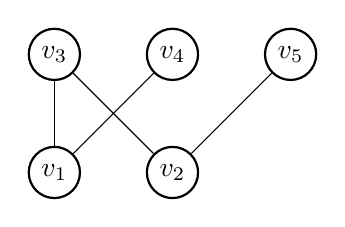
\begin{tikzpicture}
      \tikzset{
        node distance=1.5cm,
        every node/.style={circle,thick,draw,inner sep=0pt,minimum size=6.5mm}
      }

      \node[] (v1) {$v_1$};
      \node[right of=v1] (v2) {$v_2$};
      \node[above of=v1] (v3) {$v_3$};
      \node[right of=v3] (v4) {$v_4$};
      \node[right of=v4] (v5) {$v_5$};

      \draw (v1) edge[] (v3)
            (v1) edge[] (v4)
            (v2) edge[] (v3)
            (v2) edge[] (v5);
    \end{tikzpicture}
    \caption{A bipartite graph with the sets $V_1 = \{v_3, v_4, v_5\}$ and $V_2 = \{v_1, v_2\}$}
    \label{fig:graph3}
  \end{figure}
\end{minipage}\hfill
\begin{minipage}[c]{0.45\linewidth}
  \begin{figure}[H]
    \centering
    \usetikzlibrary{graphs}
    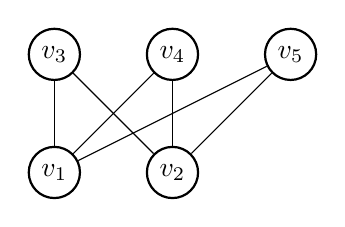
\begin{tikzpicture}
      \tikzset{
        node distance=1.5cm,
        every node/.style={circle,thick,draw,inner sep=0pt,minimum size=6.5mm}
      }
  
      \node[] (v1) {$v_1$};
      \node[right of=v1] (v2) {$v_2$};
      \node[above of=v1] (v3) {$v_3$};
      \node[right of=v3] (v4) {$v_4$};
      \node[right of=v4] (v5) {$v_5$};

      \draw (v1) edge[] (v3)
            (v1) edge[] (v4)
            (v1) edge[] (v5)
            (v2) edge[] (v3)
            (v2) edge[] (v4)
            (v2) edge[] (v5);
    \end{tikzpicture}
    \caption{A complete bipartite graph, $K_{3,2}$}
    \label{fig:graph4}
  \end{figure}
\end{minipage}

A complete bipartite graph is one in which every vertex in $V_1$ is connected to every vertex in $V_2$. This is denoted
 by $K_{m, n}$ for $\lvert V_1 \rvert = m$ and $\lvert V_2 \rvert = n$

\section*{Subgraphs}

A graph $H$ is a subgraph of graph $G$ if and only if the vertex and edge sets of $H$ are subsets of the vertex and edge
 sets of $G$, respectively. The way that the graphs are drawn is irrelevant, since any given graph could be drawn in a
 near infinite number of ways. The only thing that matters is that the structure of the graph is similar.

\begin{minipage}[c]{0.3\linewidth}
  \begin{figure}[H]
    \centering
    \usetikzlibrary{graphs}
    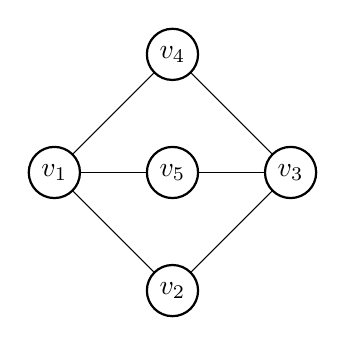
\begin{tikzpicture}
      \tikzset{
        node distance=1.5cm,
        every node/.style={circle,thick,draw,inner sep=0pt,minimum size=6.5mm}
      }
  
      \node[] (v1) {$v_1$};
      \node[right of=v1, below of=v1] (v2) {$v_2$};
      \node[right of=v2, above of=v2] (v3) {$v_3$};
      \node[right of=v1, above of=v1] (v4) {$v_4$};
      \node[right of=v1] (v5) {$v_5$};

      \draw (v1) edge[] (v2)
            (v2) edge[] (v3)
            (v3) edge[] (v4)
            (v4) edge[] (v1)
            (v1) edge[] (v5)
            (v5) edge[] (v3);
    \end{tikzpicture}
    \caption{$G$}
    \label{fig:graph5}
  \end{figure}
\end{minipage}\hfill
\begin{minipage}[c]{0.3\linewidth}
  \begin{figure}[H]
    \centering
    \usetikzlibrary{graphs}
    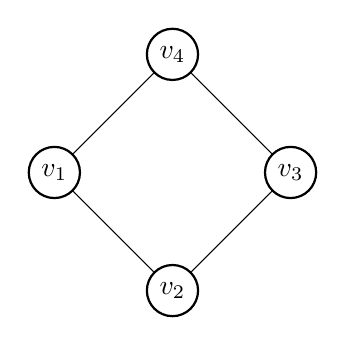
\begin{tikzpicture}
      \tikzset{
        node distance=1.5cm,
        every node/.style={circle,thick,draw,inner sep=0pt,minimum size=6.5mm}
      }
  
      \node[] (v1) {$v_1$};
      \node[right of=v1, below of=v1] (v2) {$v_2$};
      \node[right of=v2, above of=v2] (v3) {$v_3$};
      \node[right of=v1, above of=v1] (v4) {$v_4$};

      \draw (v1) edge[] (v2)
            (v2) edge[] (v3)
            (v3) edge[] (v4)
            (v4) edge[] (v1);
    \end{tikzpicture}
    \caption{$H_1$}
    \label{fig:graph6}
  \end{figure}
\end{minipage}\hfill
\begin{minipage}[c]{0.3\linewidth}
  \begin{figure}[H]
    \centering
    \usetikzlibrary{graphs}
    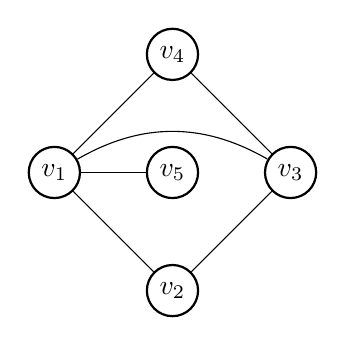
\begin{tikzpicture}
      \tikzset{
        node distance=1.5cm,
        every node/.style={circle,thick,draw,inner sep=0pt,minimum size=6.5mm}
      }
  
      \node[] (v1) {$v_1$};
      \node[right of=v1, below of=v1] (v2) {$v_2$};
      \node[right of=v2, above of=v2] (v3) {$v_3$};
      \node[right of=v1, above of=v1] (v4) {$v_4$};
      \node[right of=v1] (v5) {$v_5$};

      \draw (v1) edge[] (v2)
            (v2) edge[] (v3)
            (v3) edge[] (v4)
            (v4) edge[] (v1)
            (v1) edge[] (v5)
            (v1) edge[bend left] (v3);
    \end{tikzpicture}
    \caption{$H_2$}
    \label{fig:graph7}
  \end{figure}
\end{minipage}

In this case, $H_1$ (as in figure \ref*{fig:graph6}) is a subgraph of $G$ (as in figure \ref*{fig:graph5}), but $H_2$
 (as in figure \ref*{fig:graph7}) is not a subgraph of $G$, since it has an extra edge connecting $v_1$ to $v_3$.

\section*{Isomorphic Graphs}

There is not a terribly simple way of describing the concept of isomorphic graphs, but two graphs are isomorphic if it
 is possible to re-label the vertices of one graph to create the structure of the second graph.

\begin{minipage}[c]{0.3\linewidth}
  \begin{figure}[H]
    \centering
    \usetikzlibrary{graphs}
    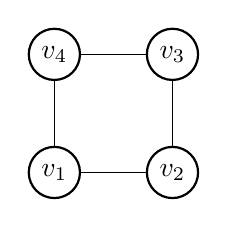
\begin{tikzpicture}
      \tikzset{
        node distance=1.5cm,
        every node/.style={circle,thick,draw,inner sep=0pt,minimum size=6.5mm}
      }
  
      \node[] (v1) {$v_1$};
      \node[right of=v1] (v2) {$v_2$};
      \node[above of=v2] (v3) {$v_3$};
      \node[above of=v1] (v4) {$v_4$};

      \draw (v1) edge[] (v2)
            (v2) edge[] (v3)
            (v3) edge[] (v4)
            (v4) edge[] (v1);
    \end{tikzpicture}
    \caption{$G_1$}
    \label{fig:graph8}
  \end{figure}
\end{minipage}\hfill
\begin{minipage}[c]{0.3\linewidth}
  \begin{figure}[H]
    \centering
    \usetikzlibrary{graphs}
    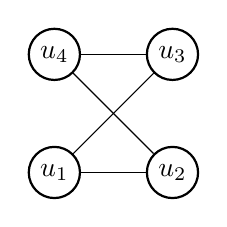
\begin{tikzpicture}
      \tikzset{
        node distance=1.5cm,
        every node/.style={circle,thick,draw,inner sep=0pt,minimum size=6.5mm}
      }
  
      \node[] (u1) {$u_1$};
      \node[right of=u1] (u2) {$u_2$};
      \node[above of=u2] (u3) {$u_3$};
      \node[above of=u1] (u4) {$u_4$};

      \draw (u1) edge[] (u2)
            (u2) edge[] (u4)
            (u4) edge[] (u3)
            (u3) edge[] (u1);
    \end{tikzpicture}
    \caption{$G_2$}
    \label{fig:graph9}
  \end{figure}
\end{minipage}\hfill
\begin{minipage}[c]{0.3\linewidth}
  \begin{figure}[H]
    \centering
    \usetikzlibrary{graphs}
    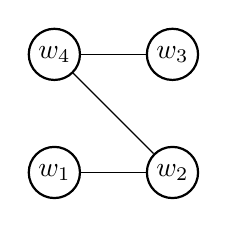
\begin{tikzpicture}
      \tikzset{
        node distance=1.5cm,
        every node/.style={circle,thick,draw,inner sep=0pt,minimum size=6.5mm}
      }
  
      \node[] (w1) {$w_1$};
      \node[right of=w1] (w2) {$w_2$};
      \node[above of=w2] (w3) {$w_3$};
      \node[above of=w1] (w4) {$w_4$};

      \draw (w1) edge[] (w2)
            (w2) edge[] (w4)
            (w4) edge[] (w3);
    \end{tikzpicture}
    \caption{$G_3$}
    \label{fig:graph10}
  \end{figure}
\end{minipage}\hfill

In this case, $G_1$ and $G_2$ are isomorphic, but $G_1$ and $G_3$ are not.\\

More formally, $G$ is isomorphic to $H$ if there is a bijective function such that $f: V(G) \rightarrow V(H)$, such that
 if $u$ and $v$ are adjacent in $G$, then $f(u)$ and $f(v)$ are adjacent in $H$, and if they are not adjacent in $G$,
 they are not adjacent in $H$ either.

It is typically very difficult to prove if two graphs are isomorphic, and as such it is usually easier to prove by
 contradiction. If $G$ and $H$ are isomorphic, then $G$ and $H$
\begin{itemize}
  \item have the same number of vertices
  \item have the same number of edges
  \item have the same degree sequence
  \item are either both connected or not connected (a topic for the next lecture)
\end{itemize}
Therefore, if any of the above are not the case, you have proven that the graphs are not isomorphic.